\documentclass[10pt]{beamer}
\usepackage[english]{babel}
\usepackage[utf8]{inputenc}
\usepackage[backend=bibtex]{biblatex}
\usepackage{graphicx}
\usepackage{caption}
\usepackage{subcaption}
\usepackage{braket}
\usepackage{csquotes}
\usepackage{diffcoeff}
\usepackage{amsmath}
\usepackage{amssymb}
\usepackage{bbold}
\usepackage{hyperref}
\usepackage{cleveref}
\usepackage{algorithm,algorithmic}
\graphicspath{{Fig/}}
\usetheme{Boadilla}
\addbibresource{ref.bib}


\author{Adhikari, Jenish}
\title{Schwinger Model}
\date{\today}
\institute{Universität Bonn}

\begin{document}
  %-------------------------------------------------------------
  \begin{frame}[plain]
    \titlepage
  \end{frame}
  %-------------------------------------------------------------
  %-------------------------------------------------------------
  \begin{frame}
    \frametitle{Table of content}
    \tableofcontents
  \end{frame}
  %-------------------------------------------------------------
 \section{Introduction}
 \begin{frame}{Introduction}
 \onslide<1-> \begin{center} \textbf{Schwinger Model}\end{center}
 \onslide<2->\begin{align}
     S[\Psi,\Psi^{\dagger},A] = \int{d^4x \{\Psi^\dagger(x)\left[i\gamma^\mu\partial_\mu +e\gamma^\mu A_\mu(x) \right]\Psi(x) +\frac{1}{4} F_{\mu\nu}F^{\mu\nu}(x) \}}
 \end{align}
     
 \end{frame}

 \section{Importance Sampling}
 \begin{frame}{Importance Sampling}
    \onslide<1-> \begin{center} \textbf{Importance Sampling}\\
        The expectation value of a physical observable $O$ is represented as \end{center}
        \begin{align}
            \braket{O} = \frac{1}{Z}\int D[\Phi]O[\Phi]e^{-S[\Phi]}
        \end{align}

 \end{frame}

 \section{Grassmann number}
 \begin{frame}{Grassmann number}
    \onslide<1-> \begin{center} \textbf{Slight detour} \end{center}
    \onslide<2-> \begin{center} \textbf{Grassmann number}\end{center} \begin{align*}
    \theta_i\theta_j &= -\theta_j\theta_i \\
    \int \Psi d\Psi & = 1\\
    \int d\Psi & = 0 \\
    \int d\Psi d\Phi {(\Psi M \Phi)} & = 0\\
    \int d\Psi d\Phi {(\Psi M \Phi)}^2 & = 2 \det(M)
    \end{align*} 
  \end{frame}

  \begin{frame}{Path Integral}
    \onslide<1->\begin{align*}
        \braket{O} &= \frac{1}{Z}\int DA D\Psi D\Phi O(A,\Psi,\Phi)e^{-S(A,\Psi,\Phi)}\\
        \braket{O} &= \frac{1}{Z}\int DA D\Psi D\Phi [O(A) + \Psi O_{\Psi\Phi}(A)\Phi]e^{-S(A) - \Psi S_{\Psi\Phi}(A)\Phi}
    \end{align*}
    \onslide<2->\begin{align*}
        \braket{O} &= \frac{1}{Z}\int DA D\Psi D\Phi [O(A) + \Psi O_{\Psi\Phi}(A)\Phi]e^{-S(A)} e^{- \Psi S_{\Psi\Phi}(A)\Phi}
    \end{align*}
    \onslide<3-> %\begin{center} No idea \end{center}
    \begin{align*}
    \braket{O} &= \frac{1}{Z}\int DA e^{-S(A)}   \{ O(A)\det(S_{\Psi\Phi}(A)) -D[\Psi\Phi] \Psi O_{\Psi\Phi}(A)\Phi\Psi S_{\Psi\Phi}(A)\Phi\}
    \end{align*}
    \onslide<4-> %\begin{center} Lecture note \end{center}
    \begin{align}\label{eqn:lecturenote}
        \braket{O} &= \frac{1}{Z}\int DA \det D_{\Psi}D_{\Phi} O_W(A)  e^{-S(A)} \\
        \det K &= \int D\eta^* D\eta e^{-\eta^\dagger K^{-1}\eta} \nonumber \\
        \braket{O} &= \frac{1}{Z}\int DA D\eta^*D\eta O_W(A)  e^{-S(A) - \eta^\dagger (D_{\Psi}D_{\Phi})^{-1} \eta} 
    \end{align}
  \end{frame}

  \begin{frame}
    \onslide<1->
    \begin{align}
        \braket{O}_{\Psi,\Phi} &= \frac{1}{Z}\int DA D\Psi D\Phi O(A,\Psi,\Phi)e^{-S(A,\Psi,\Phi)}\nonumber\\ 
        &= \frac{1}{Z}\int DA D\Psi D\Phi D\pi O(A,\Psi,\Phi)e^{\frac{1}{2}\pi^2 -S(A,\Psi,\Phi)}\nonumber\\
        &= \braket{O}_{\Psi,\Phi,\pi}
    \end{align}
    \onslide<2-> \begin{align}
        H = \frac{1}{2}\pi^2 -S(A,\Psi,\Phi)
    \end{align}
 \end{frame}
 
 \section{Discretization}
 \begin{frame}{Lattice}
    \begin{figure}
    \centering
    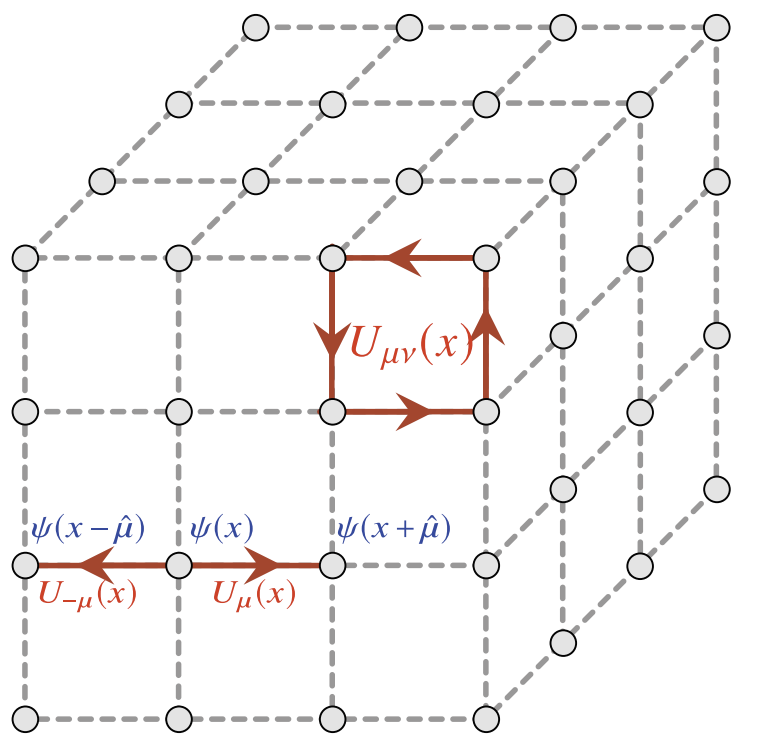
\includegraphics[width=0.45\textwidth]{lattice.png}
    \caption{Visual representation of lattice discretization: fermion fileds $\Psi(x)$ (blue) living on the sites and gauge fields as link variables $ U_{\mu}(x)$~\cite{gattringer2009quantum}}
    \end{figure}
 \end{frame}

 \begin{frame}{Plaquette}
    \begin{figure}
        \centering
        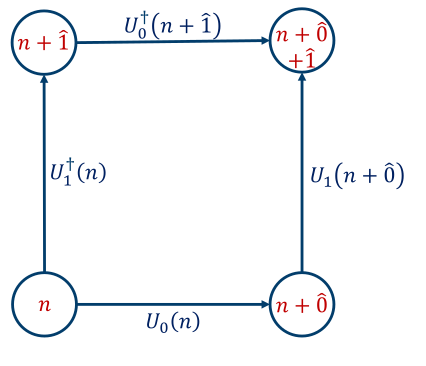
\includegraphics[width=0.45\textwidth]{plaquette.png}
        \caption{Visual representation of plaquette: $U_{\mu}(x)$~\cite{lecturenote}}
    \end{figure}
 
 \end{frame}



 \begin{frame}{Discretization}
    \onslide<1-> \begin{center} \textbf{Wilson gauge}\end{center}
    \onslide<2-> \begin{align}
        S_G(U) = \beta\sum\limits_{n\in\Lambda}\mathbb{R}\big(\mathbb{1} - P[U]_{\mu_x\nu_t}(n)\big)
    \end{align}
    \onslide<3-> \begin{center} \textbf{Wilson fermion}\end{center}
    \onslide<4-> \begin{align}
        M[n',n]^{\alpha\beta} = (m_0+2)\delta^{\alpha\beta}\delta_{n',n} -\frac{1}{2}\sum\limits_{\mu=0}^{1}\{(1-\sigma_\mu)^{\alpha\beta}U_{\mu}(n')\delta_{n'+\mu,n} &+ \nonumber\\
        (1+\sigma_\mu)^{\alpha\beta}U^{\dagger}_{\mu}(n-\mu)\delta_{n'-\mu,n}  \}\\
        M^{\dagger}[n',n]^{\alpha\beta} = (m_0+2)\delta^{\beta\alpha}\delta_{n',n} -\frac{1}{2}\sum\limits_{\mu=0}^{1}\{(1-\sigma_\mu)^{\beta\alpha}U^{\dagger}_{\mu}(n')\delta_{n'+\mu,n} &+  \nonumber \\
        (1+\sigma_\mu)^{\beta\alpha}U_{\mu}(n'-\mu)\delta_{n'-\mu,n}  \}
    \end{align}

 \end{frame}

 \begin{frame} {Lecturenote}
    \onslide<1-> \begin{center}
        On Schwinger.pdf equation 4 there should be n' on first $U$.
    \end{center}
   \onslide<2-> \begin{align}
        M^{\dagger}[n',n]^{\alpha\beta} = (m_0+2)\delta^{\beta\alpha}\delta_{n',n} -\frac{1}{2}\sum\limits_{\mu=0}^{1}\{(1-\sigma_\mu)^{\beta\alpha}U^{\dagger}_{\mu}(n)\delta_{n+\mu,n'} &+  \nonumber \\
        (1+\sigma_\mu)^{\beta\alpha}U_{\mu}(n-\mu)\delta_{n-\mu,n'}  \}\end{align}
    \onslide<3-> \begin{center}
            \textbf{Didn't give expected result for $D,D^{\dagger}$ i.e. diagonal elements}\end{center}
    \onslide<4->\begin{align}
        M^{\dagger}[n',n]^{\alpha\beta} = (m_0+2)\delta^{\beta\alpha}\delta_{n',n} -\frac{1}{2}\sum\limits_{\mu=0}^{1}\{(1-\sigma_\mu)^{\beta\alpha}U^{\dagger}_{\mu}(n')\delta_{n'+\mu,n} &+  \nonumber \\
        (1+\sigma_\mu)^{\beta\alpha}U_{\mu}(n'-\mu)\delta_{n'-\mu,n}  \} 
    \end{align}\begin{center}
        \textbf{Didn't give expected result for $D,D^{\dagger}$ i.e. diagonal elements}\end{center}
    
    
 \end{frame}

\begin{frame}
    \onslide<1->\begin{equation}
        S[\Psi,\Psi^{\dagger},A] = \int{d^4x \{\Psi^\dagger(x)\left[i\gamma^\mu\partial_\mu + e\gamma^\mu A_\mu(x) \right]\Psi(x) +\frac{1}{4} F_{\mu\nu}F^{\mu\nu}(x) \}} 
    \end{equation}
    \onslide<2->\begin{align}
        H &= \frac{\pi^2}{2} + S_G(U) + \eta^\dagger (MM^\dagger)^{-1}\eta \\
        \dot\pi & = - \diffp{H}{U} \\
        \dot U &= \diffp{H}{U} = \pi \\ \end{align} \end{frame}

\begin{frame}

    \begin{equation}
        \begin{gathered}
        F_\mu(\textbf{n}) \equiv \frac{\partial \mathcal{H}(U,\pi)}{\partial \omega_{\mu}(\textbf{n})}
                 = \\ F^{gauge}_{\mu}(\textbf{n})
                 - \left( \left(M M^\dagger\right)^{-1} \Phi \right)^\dagger \cdot
                 \left[ \frac{\partial M}{\partial \omega_{\mu}(\textbf{n})} M^\dagger + M\frac{\partial M^\dagger}{\partial \omega_{\mu}(\textbf{n})}\right] \cdot
                 \left( \left(M M^\dagger\right)^{-1} \Phi \right)
        \end{gathered}
        \end{equation}
        
    \begin{align}
        \diffp{S_G(U)}{U} =& - \beta \Im[U_\mu(n)K_\mu(n)]
    \end{align}
    \begin{align}
        \diffp{S_f(U)}{U} = -& \beta \Im[\chi^\dagger(n)\cdot(1-\sigma_\mu)\cdot U_\mu(n)\xi(n+\mu) \\ 
                            -&\chi^\dagger(n+\mu)\cdot (1+\sigma_\mu)\cdot U_\mu^\dagger(n)\xi(n)]\end{align}
    
\end{frame}
\begin{frame}
    \begin{center}
        where
    \end{center}
    \begin{align}
        K_{\mu}(n) = &U_{\nu}(n+\mu) \cdot U_{\mu}^\dagger(n+\nu) \cdot U_{\nu}^\dagger(n)  \\
                    +& U_{\nu}^\dagger(n+\mu-\nu) \cdot U_{\mu}^\dagger(n-\nu) \cdot U_{\nu}(n-\nu)\vert_{\nu\neq\mu}
    \end{align}
    \begin{align}
        \chi &= (MM^\dagger)^{-1}\Phi\\
        \xi &= M^\dagger(MM^\dagger)^{-1}\Phi
    \end{align}
\end{frame}

\begin{frame}{Symplectic integrators}
    \begin{center} Leapfrog \end{center}
    \begin{align}
        r(t+\frac{\Delta t}{2}) &= r(t) + \frac{\Delta t}{2} p(t) \\
        p(t+\Delta t) &= p(t) +\Delta t f\left(r(t+\frac{\Delta t}{2})\right) \\
        r(t+\Delta t) &= r(t+\frac{\Delta t}{2}) + \frac{\Delta t}{2}p(t+\Delta t)
    \end{align}
    
\end{frame}


\begin{frame}{Hybrid Monte Carlo Algorithm}
    \begin{itemize}
       \item Generate random lattice: $U \sim \mathcal{N}(0,1)  $
       \item \textbf{While} Sweeps $\leq  N $ \textbf{do:}
        \begin{itemize}
            \item Generate random momentum: $\pi \sim \mathcal{N}(0,1) $
            \item Generate random state: $\chi \sim \mathcal{N}(0,1) $
            \item Compute pseudofermion: $\phi = M \chi $
            \item Compute inverse using CG-Algorithm
            \item Compute Hamiltonian: $H(\phi,U,\pi)$
            \item Compute proposal $U,\pi$ with leapfrog
            \item Compute inverse using CG-Algorithm
            \item Compute New\_Hamiltonian
            \item Compute $\Delta H$
       \end{itemize}
       \item \textbf{If} $\Delta H \leq 0$ or $\mathcal{R}< e^{-\beta dE}$                                 $\mathcal{R} \in \mathcal{U}[0,1]$
        \begin{itemize}
            \item Accept state 
            \item Compute observable
            \item Compute acceptance rate
        \end{itemize}
    \end{itemize}
\end{frame}
        


\begin{frame}
    \begin{center}
        !!! Thank you for your attention !!!!
    \end{center}
        
\end{frame}

\begin{frame}[noframenumbering,plain,allowframebreaks]{Literatur}
    \printbibliography
\end{frame}

\end{document}